% !TeX root = ../thuthesis-example.tex

\chapter{数据准备与深度学习方法构建}

上一章中,我们对行人在实际地面的位置进行了二维高斯概率分布建模,而在这一章中,我们将利用层次聚类的方法融合不同摄像头的数据,并利用深度学习网络对WildTrack数据集场景进行学习,最终得到更精确的行人位置估计结果。

\section{层次聚类方法}

在上文中的二维高斯概率分布建模中,对于每个行人每个摄像头的数据均进行了一次建模过程。因此,对于每个行人的位置,有来自多个摄像头的二维高斯概率分布来建模其在特定摄像机视角下的位置概率分布。于是,我们需要对每个行人将其来自多个摄像头的位置概率进行融合,最终可得到一个确定的预测点。以此点与真实地面坐标的差异为指标,可以反向优化前述二维高斯概率分布建模时和数据融合时的超参数。令预测点与真实地面坐标的差异趋于最小值,则可得到最优的超参数。利用此最优超参数生成后续神经网络输入的热图,可以最大化神经网络方法的效果。

本文中对于相同行人来自不同摄像头的二维高斯概率分布建模融合方式为层次聚类的方法,其优势主要是模型的解释能力比较强。层次聚类包含两种方式,即凝聚型层次聚类和分裂型层次聚类。本文中使用自下而上的凝聚型算法,其核心原理是:将每个二维高斯概率分布作为初始节点,初始假设每个节点都是一类,每一次迭代将会聚合最相近的两个点或聚类,当所有点或聚类都合并成一类或者满足停止条件时,则终止模型迭代,此时便得到了聚类结果。

在聚类过程中,我们采用了Alejandro López-Cifuentes\cite{A2018Semantic}等人提出的在融合地面点时的两个约束条件。即,属于同一个行人的所有二维高斯概率分布都需满足:
\begin{enumerate}
    \item 来自不同的摄像机(因为每帧中一个行人只可能出现一次);
    \item 二者之间距离必须低于阈值$t_{g}$。
\end{enumerate}
同时,在层次聚类时,有三种聚类间距离的计算方式,分别为Single-Linkage,Complete-Linkage和Average-Linkage。
\begin{itemize}
    \item Single-Linkage:将两个不同聚类的数据点中距离最近的两个数据点间的距离作为这两个聚类之间的距离。这种方法的缺陷是,极端值很容易对聚类结果产生影响,造成一些不合理的数据聚合。两个距离并不近的聚类,可能会因为其中两个极端点距离过近而融合,影响最终聚合效果;
    \item Complete-Linkage:将两个不同聚类的数据点中距离最远的两个数据点间的距离作为这两个组合数据点的距离。这种方法的缺陷与Single-Linkage类似,也是极端值容易影响聚类效果。例如两个距离比较近的的聚类,可能由于其中的极端值距离较远而无法聚类;
    \item Average-Linkage:这种距离的计算方法是计算两个聚类的每个数据点与其他所有数据点的距离,将所有距离均值作为两个聚类间距离。这种方法计算量比较大,但结果比前两种方法更合理。
\end{itemize}
因此,本文层次聚类中选择了更合理的Average-Linkage。同时,二维高斯概率分布之间的距离若直接用中心点之间的距离来衡量,则会损失其所估计的位置概率信息,于是本文采用相对熵(Relative Entropy),又被称为KL散度(Kullback-Leibler Divergence),来度量两个概率分布(Probability Distribution)间差异。在信息理论中,相对熵等于两个概率分布的信息熵(Shannon Entropy)的差值。设$P(x), Q(x)$是随机变量$X$上的两个概率分布,在连续随机变量的情形下,相对熵的定义为:
\begin{equation}
  \text{KL}(P\|Q)=\int P(x)log{\frac{P(x)}{Q(x)}}dx
\end{equation}
但由于此处所有概率分布均为二维高斯概率分布,故它们之间的KL散度可以方便地用下式来计算:
\begin{equation}
  \begin{aligned}
  \text{KL}&\left(N(x|\bm{\mu_1},\Sigma_1)|N(x|\bm{\mu_2},\Sigma_2)\right) \\
  &=\frac{1}{2}\left[log{\frac{|\Sigma_2|}{|\Sigma_1|}}-K+tr(\Sigma_2^{-1}\Sigma_1)+(\bm{\mu_1}-\bm{\mu_2})^\top\Sigma_2^{-1}(\bm{\mu_1}-\bm{\mu_2})\right]
  \end{aligned}
\end{equation}
其中,$N(x|\bm{\mu_1},\Sigma_1)$为$\bm{\mu}=\mu_1, \Sigma=\Sigma_1$的二维高斯概率分布,$N(x|\bm{\bm{\mu_2}},\Sigma_2)$为$\bm{\mu}=\bm{\mu_2}, \Sigma=\Sigma_2$的二维高斯概率分布。最后,由于相机有重叠的视野,利用KL散度作为不同数据点之间的距离进行层次聚类后,需要摒弃只有一个数据点的聚类,通过这种方法,减少了错误聚类的数量,提升了聚类效果。

\section{深度学习数据准备}

对二维高斯概率分布进行聚类融合之后,接下来需要生成适用于后续神经网络输入和输出的图片。对于输入,本文将前述得到的二维高斯概率分布投影到一张大小为$224\times672$的热图(Heatmap)中,便于神经网络处理。为了得到最优的热图,需要对前述生成二维高斯概率分布的超参数进行调整。调整的方法是,令层次聚类得到的聚类中心点与真实地面坐标的差异趋于最小值,在此过程中进行参数记录,则可得到最优的超参数。

接下来,使用上述参数得到二维高斯概率分布后,将其投影到热图中。而输入神经网络中的真值标签图,则可以使用真实地面坐标的占据图(Occupancy Map)\cite{fleuret2007multicamera}表示。最终所得热图如图~\ref{heatmap}所示,标签图如~\ref{occupancyMap}所示。

最后,在输入神经网络前,还需要划分数据集。本文将上文中数据集扩充时通过提取的视频帧作为训练集,将官方提供的400帧图片集作为测试集。

\begin{figure}
    \centering
    \subcaptionbox{热图\label{heatmap}}
      {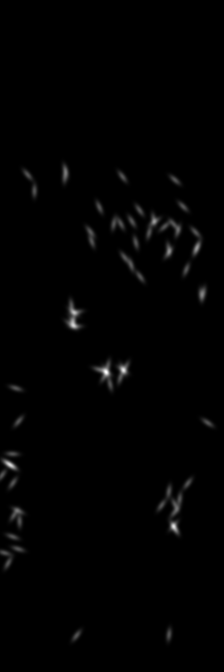
\includegraphics[width=0.2\linewidth]{frame1_heatmap.png}}
      \quad
    \subcaptionbox{标签图\label{occupancyMap}}
      {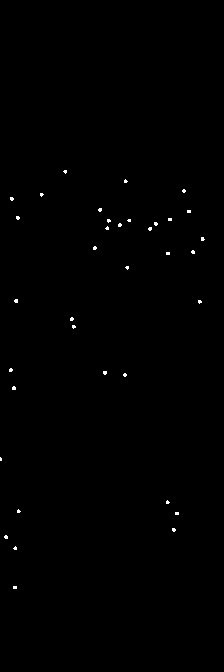
\includegraphics[width=0.2\linewidth]{frame1_occupancyMap.png}}
    \caption{神经网络输入与标签}
    \label{inputs_outputs}
\end{figure}



\section{深度学习神经网络}

\subsection{神经网络选择}

现在,我们的目标是利用深度学习算法对输入的位置概率特征进行学习,最终得到能够准确得到行人的位置。具体来说,即输入高斯概率分布热图,输出对应行人位置的占据图(Occupancy Map)。目前,在图像分析领域,深度学习方法实现的语义分割取得了很大的进展\cite{2016V, 2015U, 2017Road},本文也拓展了语义分割在行人位置估计上的应用。在生物医学应用的语义分割领域,一种流行的深度学习体系结构是U-Net\cite{2015U},它在2015年ISBI细胞跟踪挑战上达到了最好的性能,而ResUNet(Residual U-Net)\cite{2017Road}结构作为U-Net结构的改进,在道路图像提取中达到了最优的性能。同时,ResUNet++\cite{2019ResUNet}以ResUNet为基础发展而来,在医学图像分割领域取得了很不错的效果。本文基于以上进展,将上述网络作为本文工作的基础,实现了ResUNet和ResUNet++两种架构,将其作为多摄像头多目标行人位置估计的深度学习方法部分。

\subsection{神经网络结构}

本文所实现的ResUNet使用了U-Net、残差块等结构(Residual Units),而ResUNet++则在ResUNet的基础上加入了挤压和激励单元(Squeeze and Excitation Units)、空洞空间金字塔池化(Atrous Spatial Pyramid Pooling, ASPP)和注意力机制(Attention Units),从而提升了效果。下文对这些结构一一介绍,并阐明其在网络中的作用。

U-Net:在语义分割中问题中,保留高级语义信息的同时必须使用低级语义信息,这样才能保证较好的效果。然而,训练这样一个同时使用高级和低级语义信息的深层次的神经网络有很大困难,这是由深度学习网络的特点造成的。解决此问题的一种方法是Long等人\cite{2015Fully}提出的先使用预训练网络,然后在目标数据集上对其进行调整。而另一种方法则是采用U-Net\cite{2015U}中使用的数据扩充方法。此外,U-Net的体系结构也有助于缓解训练的困难,这是因为将低级特征复制到相应的高级特征上,实际上创建了一条信息传播路径,允许信号更容易地在低级和高级特征之间传播。这样不仅有助于训练的反向传播过程,而且还可以将低级特种中的细节补偿到高级语义特征上去。这种特点和ResNet\cite{he2016deep}中提出的的Residual Units原理很相似。可见,U-Net结构是一种适合本文中最后部分位置估计的网络基础结构。

残差块(Residual Units):在ResNet网络提出之前,传统的卷积神经网络都是通过将一系列卷积层与池化层进行堆叠得到的。一般认为,网络越深,特征信息越丰富,模型效果应该越好。但是实验证明,效果并非如此。这是因为当网络深度堆叠到一定程度时,会发生梯度消失或梯度爆炸的问题和退化问题(Degradation Problem)\cite{he2016deep}。因此,何凯明等人提出了残差块来解决此问题。残差块的功能可由下式表示:
\begin{equation}
    \begin{split}
    \mathbf{y}_{l}\ \ \ & = h(\mathbf{x}_{l})+\mathcal{F}(\mathbf{x}_{l}, \mathcal{W}_{l}), \\
    \mathbf{x}_{l+1} & = f(\mathbf{y}_{l}),
    \end{split}
\end{equation}
其中,$\mathbf{x}_{l}$和$\mathbf{x}_{l+1}$是第$l$个残差单元的输入和预测,$\mathcal{F}(\cdot)$为残差函数,$f(\mathbf{y}_l)$是激活函数,$h(\mathbf{x}_{l})$是恒等映射函数,例如$h(\mathbf{x}_{l}) = \mathbf{x}_{l}$这样的函数就是恒等映射函数。在一个残差块中,有以不同方式组合的批标准化(Batch Normalization),ReLU激活函数和卷积层,而本文中采用了何凯明\cite{he2016deep}提出的综合性能最好的组合方式,图~\ref{residual_compare}展示了未采用残差块与采用残差块的对比,同时展示了所采用残差块的结构。
\begin{figure}
    \centering
    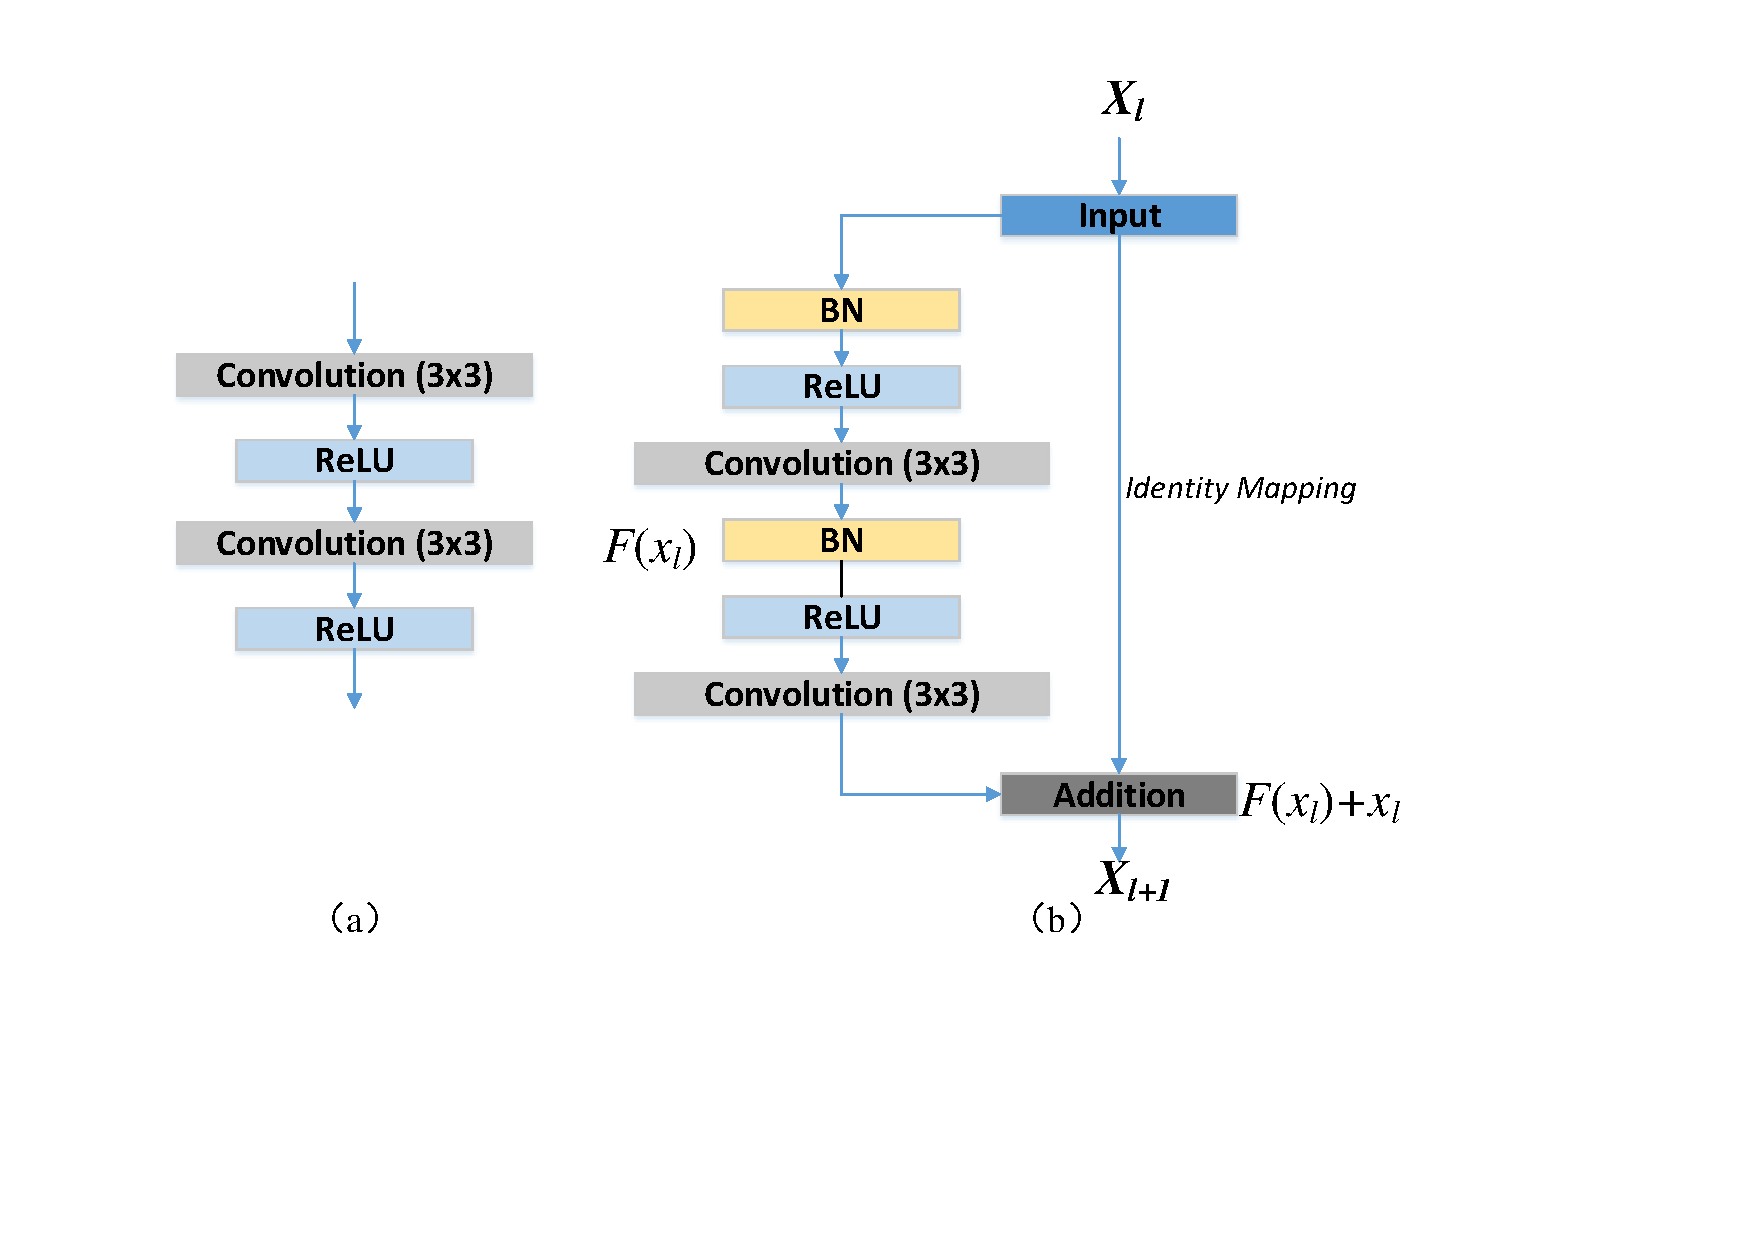
\includegraphics[width=0.5\linewidth]{res-u-net-blocks.pdf}
    \caption{(a)未采用残差块与(b)采用残差块的对比}
    \label{residual_compare}
\end{figure}

ResUNet:结合上述U-Net和残差块的技术,可以构建ResUNet网络\cite{2017Road}。这种结合可以带来两个优势:1)残差块使得可以构建的网络深度大大增加;2)残差块内部和网络高、底层次之间的直接连接大大减少了信息传播中的退化现象,从而在提高效果的同时还可以减少网络参数。本文所实现的ResUNet网络结构如图~\ref{Net_a}所示。网络采用了七层结构,为自编码器结构,主要分为编码层、中间层和解码层。编码层将输入的图片编码为压缩抽象表示,而解码层将压缩抽象表示解码为与输入大小相同的输出图片,中间层主要起到连接编码层和解码层、传输特征的作用。
\begin{figure}
    \centering
    \subcaptionbox{ResUNet网络结构\cite{2017Road}\label{Net_a}}
      {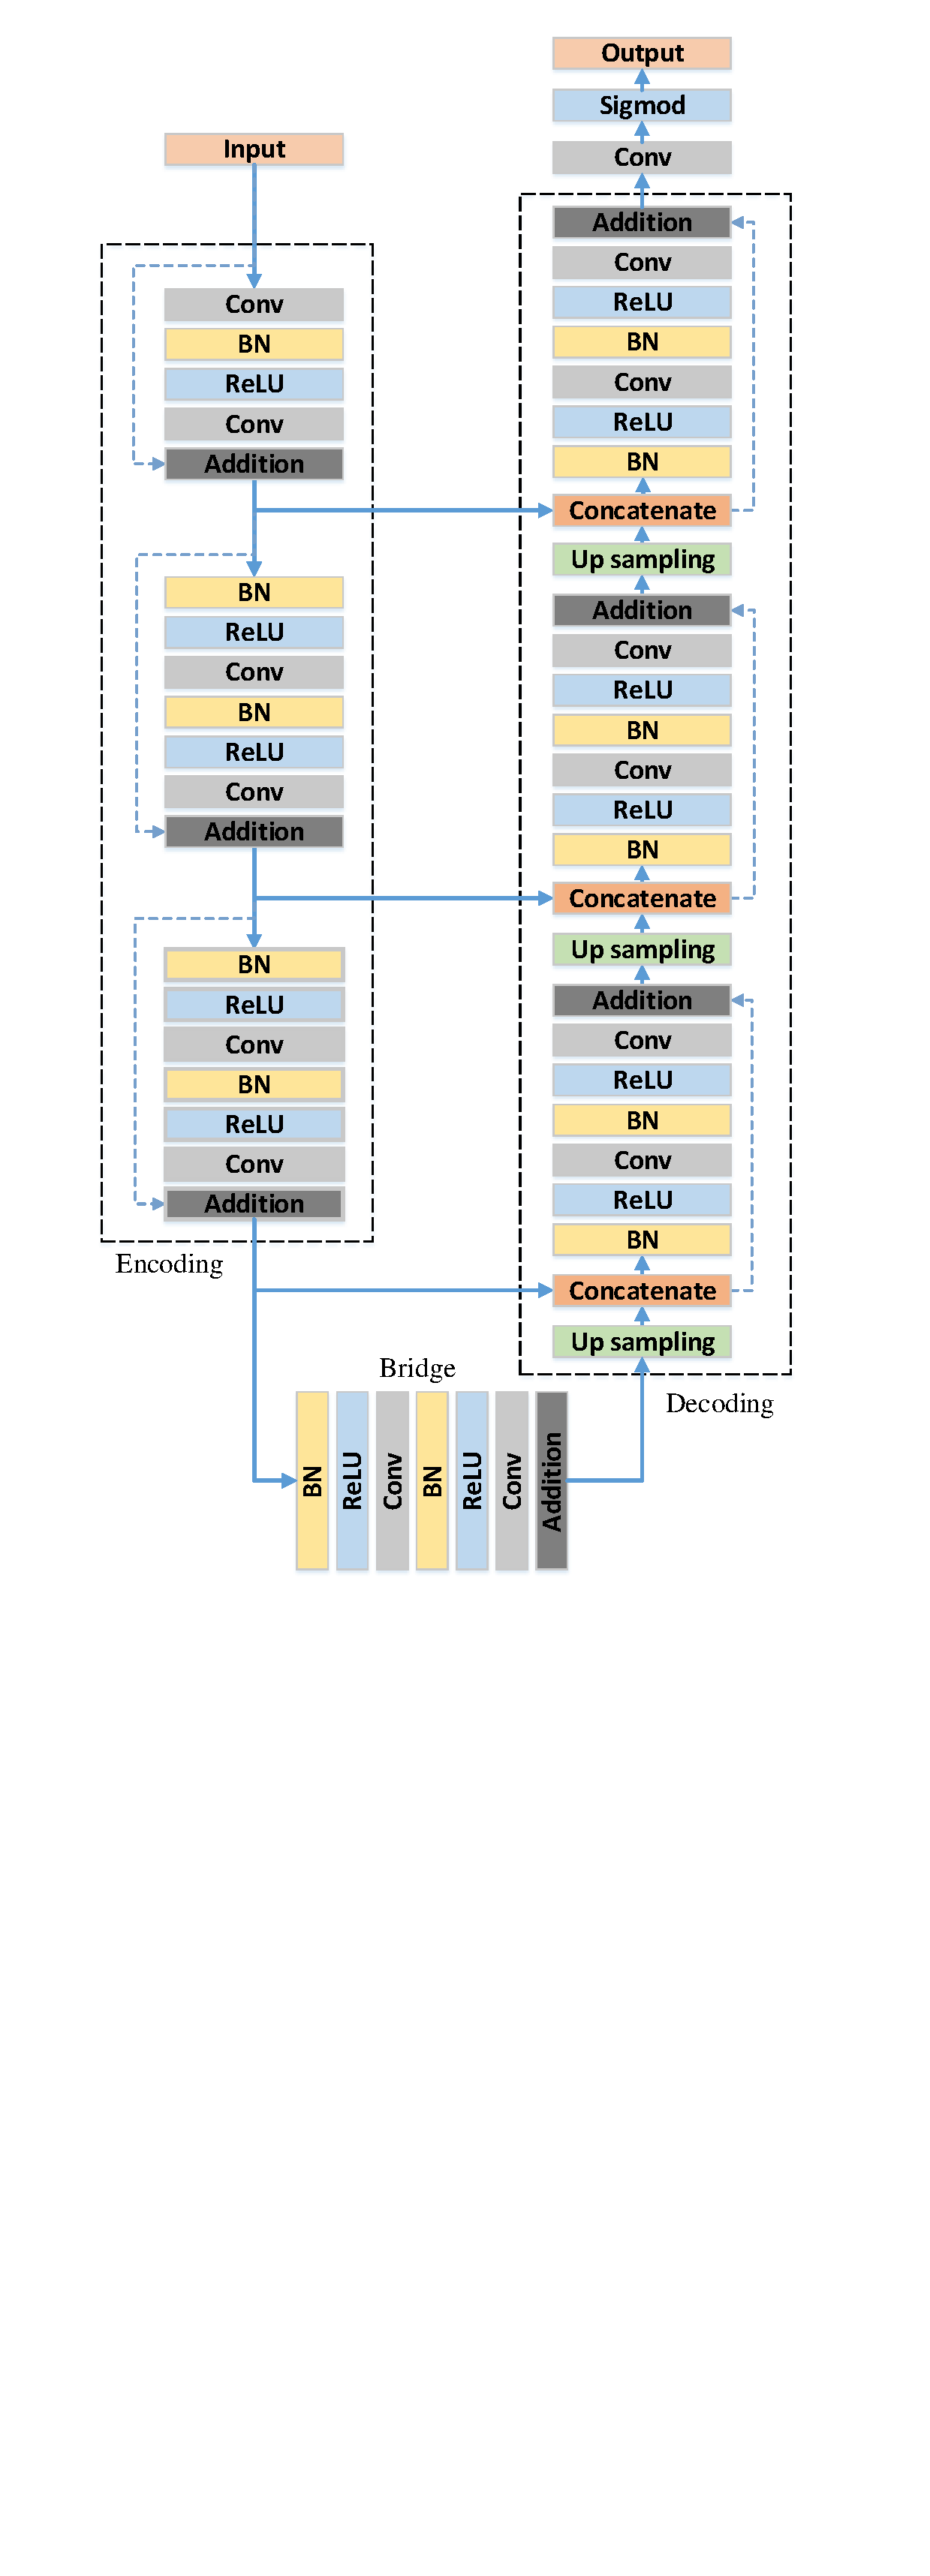
\includegraphics[width=0.36\linewidth]{ResUNet.pdf}}
    \subcaptionbox{ResUNet++网络结构\cite{2019ResUNet}\label{Net_b}}
      {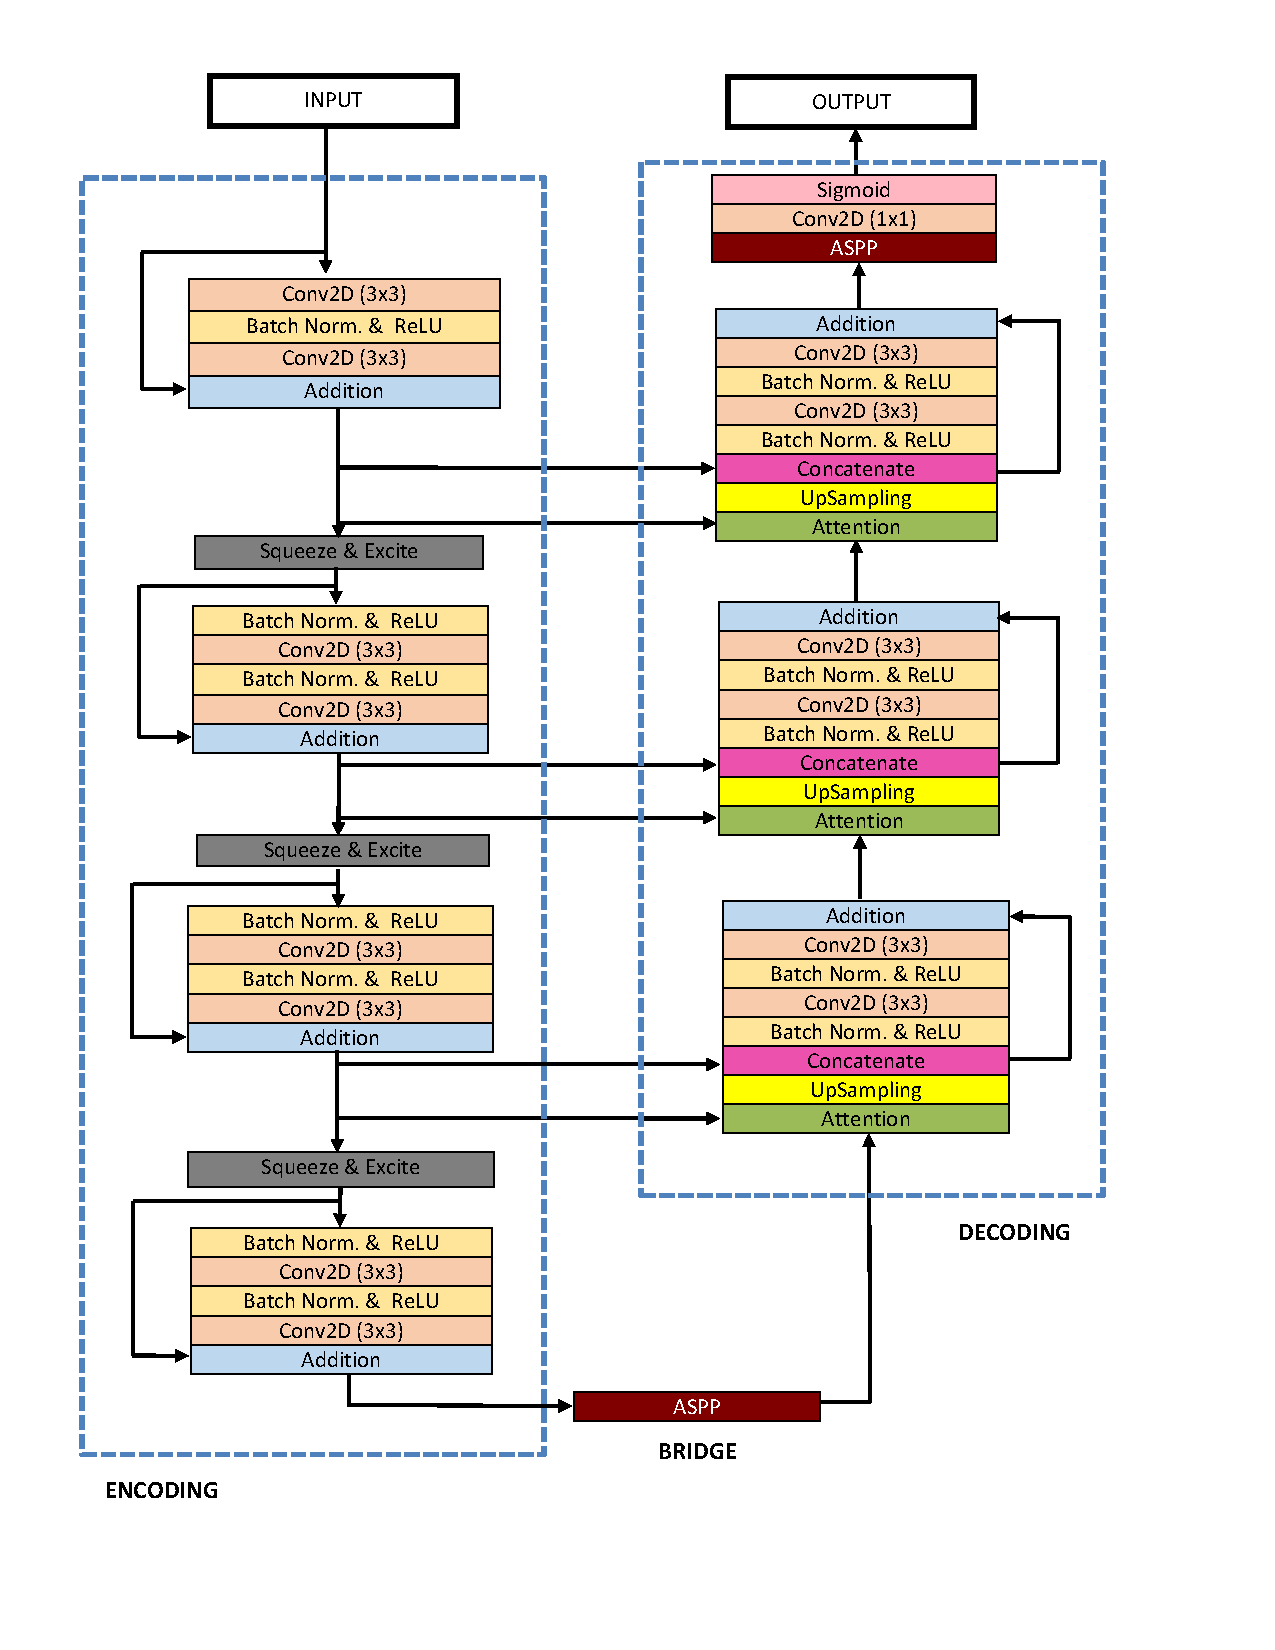
\includegraphics[width=0.62\linewidth]{ResUNet++.pdf}}
    \caption{本文实现的两种神经网络结构}
    \label{Net}
\end{figure}

挤压和激励单元(Squeeze and Excitation Units):挤压和激励网络(Squeeze-and-Excitation Networks)\cite{2017Squeeze}通过精确建模网络中通道的相互依赖关系,以及校准特征的方法,大大提高了网络的表示性能。因此,本文所采用的ResUNet++中也使用了挤压和激励单元,其主要目的是提高网络对关注特征的敏感性,抑制不必要特征。正如其名,挤压和激励单元实施的操作为先挤压全局信息并通过全局平均池(Global Average Pooling)来生成信息,然后激励以得到通道之间的相关性。

空洞空间金字塔池化(Atrous Spatial Pyramid Pooling, ASPP):何凯明等人\cite{2014Spatial}提出的ASPP方法,使得网络可以控制视野从而精确捕获多个尺度的信息。在本文实现的ResUNet++中,ASPP主要作为编码器和解码器之间的中间层,其作用主要是为语义分割提取多尺度的信息。

注意力机制(Attention Units):注意力机制实质上是一种分配机制,其核心思想是突出对象的某些重要特征,使得网络能够根据对象的重要程度重新分配资源。注意力机制的主要优势是可以被简单地运用在任何尺寸的输入中,显著提升特征的质量,从而促进效果的提升。在本文实现的ResUNet++中,注意力机制被加入到解码器的部分,从而使得网络能够专注于特征图中的关键区域。

ResUNet++:结合上述挤压和激励单元、空洞空间金字塔池化和注意力机制,在ResUNet的基础上,本文实现了ResUNet++网络。网络也分为七层结构,与ResUNet的结构基本一致,但加入了挤压和激励单元、空洞空间金字塔池化和注意力机制,从而大大提升了网络的预测效果。

\subsection{损失函数}

在构建的ResUNet和ResUNet++两个深度学习神经网络中,本文均采用了二进制交叉熵(Binary Cross Entropy, BCE)损失和Dice系数(Dice Coefficient)损失相结合的损失函数。二进制交叉熵可由下式计算:
\begin{equation}
  \mathcal{L}_{BCE} = \frac{1}{N}\sum_{n=1}^{N}l_{n}
\end{equation}
其中,$l_n=-w[y_n \cdot log{x_n}+(1-y_n) \cdot log(1-x_n)]$为第$n$个样本对应的loss,其中$w$为超参数。在本文中,上式loss体现为将预测图的第n个像素作为样本,标签图的第n个像素作为样本标签的loss。而Dice系数是一种集合相似度度量函数,通常用于计算两个样本的相似度。Dice系数损失的计算可由下式得到:
\begin{equation}
  \mathcal{L}_{Dice} = 1-\frac{2|X \cap Y|}{|X|+|Y|}
\end{equation}
其中,$X$为预测图,$Y$为标签图,$|X \cap Y|$是$X$和$Y$之间的交集,$|X|$和$|Y|$表示$X$和$Y$的元素的个数。在实际计算时,$|X \cap Y|$近似为预测图和标签图之间的点乘,并将点乘的元素的结果逐元素相加。而计算$|X|$和$|Y|$时,本文采取了直接进行逐元素相加的方式。

最终,将两种损失结合起来,就得到了本文所采用的损失函数,如下:
\begin{equation}
  \mathcal{L} = \mathcal{L}_{BCE} + \mathcal{L}_{Dice}
\end{equation}

\section{本章小结}

本章中介绍了构建层次聚类方法得到粗略的行人位置估计和通过粗略的估计结果反向优化高斯概率分布和层次聚类的超参数的过程,然后介绍了利用扩充和预处理后得到的数据如何被用来制作适合网络输入的热图和标签图。最后,详细阐述了本文所实现的ResUNet和ResUNet++两种深度学习神经网络结构和所采用的损失函数。这两种深度学习方法将输出行人位置估计的更准确的预测,可以作为本文工作中的估计结果。